\begin{figure}[!h]
    \centering
    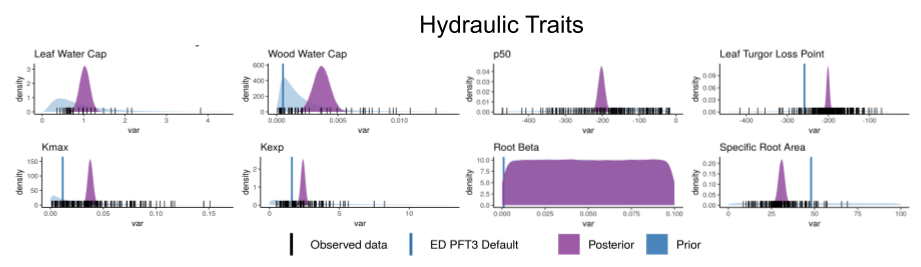
\includegraphics[width=.95\textwidth]{Hydro_Paper_LaTeX/Hydro_Paper_Figures/hydraulic_traits.png}
    \caption[Hydraulic Traits]{Parameter distributions for ED2-hydro PFT in the BETY database. Prior distributions (blue) were constrained by data from BETYdb (not pictured, though in the final version of the plot I do want to have data points) using Bayesian meta-analysis to produce posterior distributions (purple). In two cases there was no data to constrain the prior and thus the posterior remains uninormative. The dashed dark blue line shows the default value for ED2-hydro's mid-successional tropical PFT.
    \todoq{Because my PFT is a combination of early, mid and late, would it be useful or clutter to have all three PFT default lines on the plot? Are the default lines useful at all?}
    }
    \label{fig:hydraulic_traits}
\end{figure}